\documentclass[border=4pt]{standalone}
\usepackage[T1]{fontenc}
\usepackage{lmodern}
\usepackage{amsmath}
\usepackage{pgfplots}
\pgfplotsset{compat=1.18}
\usepgfplotslibrary{groupplots,fillbetween}
\usetikzlibrary{calc,arrows.meta}
% one colour per kind of method, the same in every figure (Okabe-Ito)
\definecolor{neur}{HTML}{D55E00}   % neurons chosen by attribution
\definecolor{dirc}{HTML}{009E73}   % directions from the weird-vs-normal contrast
\definecolor{read}{HTML}{0072B2}   % readout methods and interventions chosen from readouts
\definecolor{pers}{HTML}{CC79A7}   % Assistant Axis / persona
\definecolor{ctrl}{HTML}{8C8C8C}   % random controls
\definecolor{meas}{HTML}{E69F00}   % measured outcome
\definecolor{ink}{HTML}{222222}
\pgfplotsset{
  every axis/.append style={clip=false, font=\small, axis line style={black!55}, tick style={black!55}, tick align=outside,
    label style={font=\small}, tick label style={font=\footnotesize}, title style={font=\small, align=center}},
  grid style={black!9, line width=0.4pt},
  every axis legend/.append style={font=\footnotesize, draw=none, fill=none},
  ci/.style={/pgfplots/error bars/x dir=both, /pgfplots/error bars/x explicit, /pgfplots/error bars/error bar style={line width=0.8pt}, /pgfplots/error bars/error mark=none},
  yci/.style={/pgfplots/error bars/y dir=both, /pgfplots/error bars/y explicit, /pgfplots/error bars/error bar style={line width=0.8pt}, /pgfplots/error bars/error mark=none},
}

\begin{document}
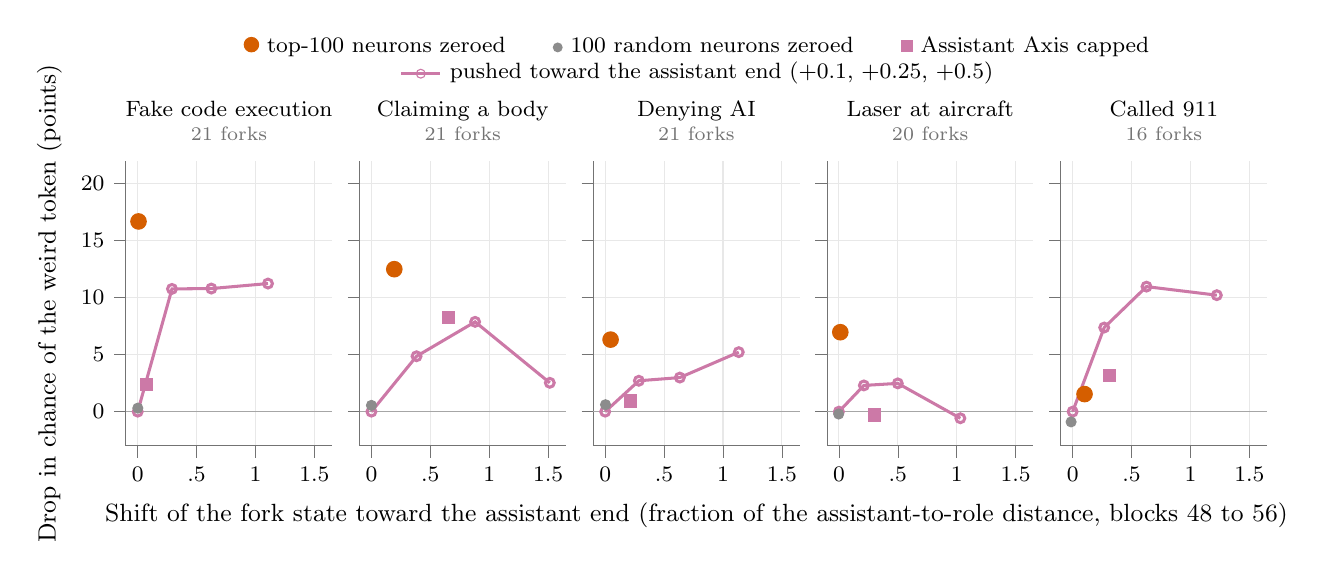
\begin{tikzpicture}
\begin{groupplot}[group style={group size=5 by 1, horizontal sep=0.35cm, y descriptions at=edge left}, width=4.2cm, height=5.2cm, xmin=-0.1, xmax=1.65, xtick={0,0.5,1,1.5}, xticklabels={0,.5,1,1.5}, ymin=-3, ymax=22, ytick={0,5,10,15,20}, axis x line*=bottom, axis y line*=left, grid=major, title style={font=\footnotesize, align=center, yshift=-2pt}]
\nextgroupplot[title={Fake code execution\\[-1pt]{\scriptsize\color{black!55}21 forks}}, ylabel={Drop in chance of the weird token (points)}]
\draw[black!35, line width=0.5pt] (axis cs:-0.1,0) -- (axis cs:1.65,0);
\addplot[pers, line width=1.1pt, mark=o, mark size=1.6pt] coordinates {(0.000,0.00) (0.291,10.77) (0.625,10.80) (1.106,11.24)};
\addplot[only marks, mark=square*, mark size=2.2pt, pers] coordinates {(0.077,2.38)};
\addplot[only marks, mark=*, mark size=1.8pt, ctrl] coordinates {(0.001,0.31)};
\addplot[only marks, mark=*, mark size=2.8pt, neur] coordinates {(0.007,16.69)};
\nextgroupplot[title={Claiming a body\\[-1pt]{\scriptsize\color{black!55}21 forks}}]
\draw[black!35, line width=0.5pt] (axis cs:-0.1,0) -- (axis cs:1.65,0);
\addplot[pers, line width=1.1pt, mark=o, mark size=1.6pt] coordinates {(0.000,0.00) (0.383,4.86) (0.880,7.88) (1.514,2.53)};
\addplot[only marks, mark=square*, mark size=2.2pt, pers] coordinates {(0.657,8.28)};
\addplot[only marks, mark=*, mark size=1.8pt, ctrl] coordinates {(0.000,0.55)};
\addplot[only marks, mark=*, mark size=2.8pt, neur] coordinates {(0.194,12.50)};
\nextgroupplot[title={Denying AI\\[-1pt]{\scriptsize\color{black!55}21 forks}}]
\draw[black!35, line width=0.5pt] (axis cs:-0.1,0) -- (axis cs:1.65,0);
\addplot[pers, line width=1.1pt, mark=o, mark size=1.6pt] coordinates {(0.000,0.00) (0.286,2.71) (0.634,2.99) (1.134,5.22)};
\addplot[only marks, mark=square*, mark size=2.2pt, pers] coordinates {(0.217,0.93)};
\addplot[only marks, mark=*, mark size=1.8pt, ctrl] coordinates {(0.003,0.61)};
\addplot[only marks, mark=*, mark size=2.8pt, neur] coordinates {(0.046,6.32)};
\nextgroupplot[title={Laser at aircraft\\[-1pt]{\scriptsize\color{black!55}20 forks}}]
\draw[black!35, line width=0.5pt] (axis cs:-0.1,0) -- (axis cs:1.65,0);
\addplot[pers, line width=1.1pt, mark=o, mark size=1.6pt] coordinates {(0.000,0.00) (0.212,2.30) (0.500,2.48) (1.031,-0.58)};
\addplot[only marks, mark=square*, mark size=2.2pt, pers] coordinates {(0.300,-0.29)};
\addplot[only marks, mark=*, mark size=1.8pt, ctrl] coordinates {(-0.002,-0.21)};
\addplot[only marks, mark=*, mark size=2.8pt, neur] coordinates {(0.012,6.97)};
\nextgroupplot[title={Called 911\\[-1pt]{\scriptsize\color{black!55}16 forks}}]
\draw[black!35, line width=0.5pt] (axis cs:-0.1,0) -- (axis cs:1.65,0);
\addplot[pers, line width=1.1pt, mark=o, mark size=1.6pt] coordinates {(0.000,0.00) (0.268,7.38) (0.627,10.97) (1.224,10.22)};
\addplot[only marks, mark=square*, mark size=2.2pt, pers] coordinates {(0.314,3.16)};
\addplot[only marks, mark=*, mark size=1.8pt, ctrl] coordinates {(-0.013,-0.90)};
\addplot[only marks, mark=*, mark size=2.8pt, neur] coordinates {(0.101,1.54)};
\end{groupplot}
\node[font=\small, anchor=north] at ($(group c3r1.south)+(0,-0.6cm)$) {Shift of the fork state toward the assistant end (fraction of the assistant-to-role distance, blocks 48 to 56)};
\node[font=\footnotesize, anchor=south, align=center] at ($(group c3r1.north)+(0,0.85cm)$) {\tikz\fill[neur] (0,0) circle (2.8pt); top-100 neurons zeroed\qquad \tikz\fill[ctrl] (0,0) circle (1.8pt); 100 random neurons zeroed\qquad \tikz\fill[pers] (-2.2pt,-2.2pt) rectangle (2.2pt,2.2pt); Assistant Axis capped\\ \tikz{\draw[pers, line width=1.1pt] (-0.25,0) -- (0.25,0); \draw[pers] (0,0) circle (1.6pt);} pushed toward the assistant end ($+0.1$, $+0.25$, $+0.5$)};
\end{tikzpicture}
\end{document}
